\documentclass[a4paper,12pt]{article}
\usepackage[utf8]{inputenc}
\usepackage[german]{babel}
\usepackage{amsmath}
\usepackage{amssymb}
\usepackage{amsthm}
\usepackage{geometry}
\usepackage{graphicx}
\usepackage[hidelinks]{hyperref}
\usepackage{listings}
\usepackage{xcolor}
\usepackage{algorithm}
\usepackage{algpseudocode}
\usepackage{chngcntr}

\geometry{margin=2.5cm}

\theoremstyle{definition}
\newtheorem{definition}{Definition}
\newtheorem{beispiel}{Beispiel}
\newtheorem{frage}{Frage}
\newtheorem{satz}{Satz}
\newtheorem{lemma}{Lemma}
\newtheorem{korollar}{Korollar}
\counterwithin{algorithm}{section}

% Code-Highlighting
\lstset{
	basicstyle=\ttfamily\small,
	keywordstyle=\color{blue},
	commentstyle=\color{gray},
	stringstyle=\color{red},
	numbers=left,
	numberstyle=\tiny,
	breaklines=true,
	frame=single
}

\title{Graphen mit Knoten und Kanten \\[0.5ex]\large Optimale Einordnung in die Graphprofilverteilung}
\author{Stephan Epp}
\date{\today}

\begin{document}

\maketitle

\tableofcontents
\newpage

\section{Einführung}

Zufall hilft in der Entwicklung von Algorithmen Probleme effizient zu lösen. Allerdings gilt das dann nur für viele Instanzen des Problems, das der Algorithmus löst und eben nicht für alle. Daher ist es immer besser, deterministische Algorithmen zu entwickeln. Denn ihre Laufzeit halten sie für alle Instanzen stets ein.

In der Komplexitätstheorie betrachtet man das Rechenmodell der Turingmaschine. Eine nichtdeterministische Turingmaschine ist eine Turingmaschine, für die es eine Eingabe gibt, bei der diese Turingmaschine sich aussucht, welches der nächste Zustand ist. Das kann sie nur deshalb, weil sie so definiert ist, dass es für diese Eingabe mehr als nur einen anderen nächsten Zustand gibt. Diese Definition befreit den Anwender dieser Maschine nicht von der Unsicherheit, was diese Maschine schließlich in einer Abarbeitungsfolge berechnet. Es ist nicht erklärbar, wie dann davon auszugehen ist, dass diese Maschine nur in einer Abarbeitungsfolge richtig rechnet.

Die Berechnung von Profilwerten für Graphen erfordert effiziente Algorithmen zur Bestimmung von Wegeigenschaften. In dieser Arbeit wird gezeigt, wie die Signatur-Methode aus der Boolean Matrixmultiplikation zur effizienten Berechnung dieser Profilwerte eingesetzt werden kann.

\section{Definitionen}
In diesem Kapitel werden die Definitionen für diese Arbeit eingeführt.
\subsection{Graphen}
\begin{definition}[Graph]
	Ein Graph $G = (V, E)$ besteht aus einer Menge von Knoten $V$ und einer Menge von Kanten $E \subseteq V \times V$.
\end{definition}

\begin{definition}[Adjazenzmatrix]
	Für einen Graphen $G = (V, E)$ mit $n = |V|$ Knoten ist die Adjazenzmatrix $A \in \{0,1\}^{n \times n}$ definiert durch:
	\[
	A_{ij} = \begin{cases} 1 & \text{falls } (i,j) \in E \\ 0 & \text{sonst} \end{cases}
	\]
\end{definition}

\subsection{Wegeigenschaften}
\begin{definition}[Weg]
	Ein Weg der Länge $k$ von Knoten $i$ zu Knoten $j$ ist eine Folge von Knoten $(v_0, v_1, \ldots, v_k)$ mit $v_0 = i$, $v_k = j$ und $(v_l, v_{l+1}) \in E$ für alle $0 \leq l < k$.
\end{definition}

\begin{lemma}[Wege und Matrixpotenzen]
	Sei $A$ die Adjazenzmatrix eines Graphen $G = (V,E)$ und $A^k$ die $k$-te Potenz von $A$ unter Boolean Matrixmultiplikation. Dann gilt:
	\[
	(A^k)_{ij} = 1 \Leftrightarrow \text{es existiert ein Weg der Länge } k \text{ von } i \text{ nach } j
	\]
\end{lemma}

\begin{proof}
	Der Beweis erfolgt durch Induktion über $k$.\newline
	\textbf{Induktionsanfang:} Für $k=1$ gilt $(A^1)_{ij} = A_{ij} = 1$ genau dann, wenn $(i,j) \in E$, also ein Weg der Länge 1 existiert.\newline
	\textbf{Induktionsschritt:} Sei die Aussage für $k$ erfüllt. Für $k+1$ gilt:
	\begin{align*}
		(A^{k+1})_{ij} &= \bigvee_{l=1}^{n} ((A^k)_{il} \wedge A_{lj}) = 1
	\end{align*}
	Dies ist genau dann erfüllt, wenn es ein $l$ gibt mit $(A^k)_{il} = 1$ und $A_{lj} = 1$. Nach Induktionsvoraussetzung existiert dann ein Weg der Länge $k$ von $i$ nach $l$ und eine Kante von $l$ nach $j$, also ein Weg der Länge $k+1$ von $i$ nach $j$.
\end{proof}

\begin{definition}[Profil]
	Das Profil eines Graphen $G=(V, E)$ besteht aus 
	\begin{itemize}
		\item[-] dem kürzesten Weg für alle Knoten $v \in V$,
		\item[-] dem längsten Weg für alle Knoten $v \in V$ und
		\item[-] dem Kantenmaß $\kappa = \frac{\left|V\right|}{\left|E\right|}$.
	\end{itemize}
\end{definition}

Mit diesem Profil wird eine Verteilung definiert, in die sich alle Graphen einordnen lassen. Ausschlaggebend für die unterschiedlichen Bereiche in der Verteilung ist die erforderliche Laufzeit der Algorithmen zur Ermittlung aller Profilwerte. Natürlich ist es dafür nötig, dass die Algorithmen die Profilwerte in optimaler Laufzeit berechnen. Sonst wäre die Einordnung nicht klar.

\begin{definition}[Erreichbarkeitsmatrix]
	Die Erreichbarkeitsmatrix $R \in \{0,1\}^{n \times n}$ eines Graphen $G$ ist definiert als:
	\[
	R_{ij} = \begin{cases} 1 & \text{falls ein Weg von } i \text{ nach } j \text{ existiert} \\ 0 & \text{sonst} \end{cases}
	\]
\end{definition}

\begin{satz}[Erreichbarkeit durch Matrixpotenzen]
	Für einen Graphen mit $n$ Knoten gilt:
	\[
	R = A \vee A^2 \vee A^3 \vee \cdots \vee A^{n-1}
	\]
	wobei $\vee$ die komponentenweise logische ODER-Operation bezeichnet.
\end{satz}

\begin{proof}
	Da der längste einfache Weg in einem Graphen mit $n$ Knoten höchstens die Länge $n-1$ hat, genügt es alle Potenzen bis $A^{n-1}$ zu betrachten. Ein Weg von $i$ nach $j$ existiert genau dann, wenn es einen Weg einer Länge $k \in \{1, \ldots, n-1\}$ gibt.
\end{proof}

Die naive Implementierung hat eine Laufzeit von $O(n^3)$. Fortgeschrittene Algorithmen wie \textsc{Strassen} (1969) oder \textsc{Coppersmith-Winograd} (1990) erreichen $O(n^{2.807})$ bzw. $O(n^{2.376})$.

Für \textbf{Boolean Matrizen}, bei denen alle Einträge $\{0, 1\}$ sind und die Operationen durch logische Operationen ersetzt werden, kann die Signatur-Technik aus dem Subgraph Algorithmus genutzt werden, um eine Laufzeit von $O(n^2)$ zu erreichen.

\begin{definition}[Boolean Matrixmultiplikation]
	Für zwei Boolean Matrizen $A, B \in \{0,1\}^{n \times n}$ ist die Boolean Matrixmultiplikation definiert als:
	\[
	C_{ij} = \bigvee_{k=1}^{n} (A_{ik} \wedge B_{kj})
	\]
	wobei $\vee$ das logische ODER und $\wedge$ das logische UND bezeichnet.
\end{definition}

Mit anderen Worten: $C_{ij} = 1$ genau dann, wenn es mindestens ein $k$ gibt mit $A_{ik} = 1$ und $B_{kj} = 1$.

\section{Algorithmen}

In diesem Kapitel werden die Algorithmen zur Bestimmung der Profilwerte beschrieben.

\subsection{Boolean Matrixmultiplikation}

Der Kerngedanke für die Arbeitsweise des Algorithmus zur Boolean Matrixmultiplikation mit Signaturen ist, jede \textbf{Zeile} von $A$ als Signatur zu kodieren und jede \textbf{Spalte} von $B$ als Signatur zu kodieren und für jedes Element Element $C_{ij}$:
\begin{itemize}
	\item[-] Berechne bitweise UND der Signaturen: $\sigma(\text{row}_i(A)) \; \& \; \sigma(\text{col}_j(B))$
	\item[-] Setze $C_{ij} = 1$ falls Ergebnis $\neq 0$, sonst $C_{ij} = 0$
\end{itemize}

Algorithmus \ref{alg:bmm} beschreibt die Arbeitsweise zur Boolean Matrixmultiplikation mit Signaturen.

\begin{algorithm}[htb]
	\caption{Boolean Matrixmultiplikation mit Signaturen}
	\label{alg:bmm}
	\textbf{Eingabe:} Zwei Boolean Matrizen $A, B \in \{0,1\}^{n \times n}$ \\
	\textbf{Ausgabe:} Boolean Matrix $C \in \{0,1\}^{n \times n}$ mit $C_{ij} = \bigvee_{k=1}^{n} (A_{ik} \wedge B_{kj})$
	\begin{algorithmic}[1]
		\State $n \gets \text{Dimension von } A$
		\State $\text{rowSig} \gets \text{leeres Array der Länge } n$
		\State $\text{colSig} \gets \text{leeres Array der Länge } n$
		\For{$i = 0$ \textbf{to} $n-1$}
		\State $\text{rowSig}[i] \gets \sum_{k=0}^{n-1} A_{ik} \cdot 2^k$ \Comment{$O(n)$}
		\EndFor
		\For{$j = 0$ \textbf{to} $n-1$}
		\State $\text{colSig}[j] \gets \sum_{k=0}^{n-1} B_{kj} \cdot 2^k$ \Comment{$O(n)$}
		\EndFor
		\State $C \gets n \times n$ Nullmatrix
		\For{$i = 0$ \textbf{to} $n-1$}
		\For{$j = 0$ \textbf{to} $n-1$}
		\State $\text{andResult} \gets \text{rowSig}[i] \; \& \; \text{colSig}[j]$ \Comment{$O(1)$ Bitoperation}
		\If{$\text{andResult} \neq 0$}
		\State $C_{ij} \gets 1$
		\EndIf
		\EndFor
		\EndFor    
		\State \Return $C$
	\end{algorithmic}
\end{algorithm}

\begin{satz}[Korrektheit der Signatur-Methode]
	Sei $r = \sigma(\text{row}_i(A))$ die Signatur der $i$-ten Zeile von $A$ und $c = \sigma(\text{col}_j(B))$ die Signatur der $j$-ten Spalte von $B$. Dann gilt:
	\begin{align}
		C_{ij} = 1 \Leftrightarrow (r \; \& \; c) \neq 0
	\end{align}
\end{satz}

\begin{proof}
	Nach Definition ist:
	\begin{align}
		C_{ij} = 1 \Leftrightarrow \exists k: A_{ik} = 1 \text{ und } B_{kj} = 1
	\end{align}
	Die bitweise UND-Operation $r \; \& \; c$ berechnet:
	\begin{align}
		r \; \& \; c = \sum_{k=0}^{n-1} (A_{ik} \wedge B_{kj}) \cdot 2^k
	\end{align}
	Dieses Ergebnis ist genau dann $\neq 0$, wenn mindestens ein Term $(A_{ik} \wedge B_{kj}) \neq 0$ ist, was äquivalent ist zu: es existiert ein $k$ mit $A_{ik} = 1$ und $B_{kj} = 1$.
\end{proof}

\begin{satz}[Laufzeit]
	Der Boolean Matrixmultiplikations-Algorithmus mit Signaturen hat eine Laufzeit von $O(n^2)$.
\end{satz}

\begin{proof}
	Der Algorithmus besteht aus zwei Phasen:\newline	
	\textbf{Phase 1: Signatur-Berechnung}
	\begin{itemize}
		\item[-] Berechnung aller Zeilen-Signaturen: $n$ Zeilen $\times$ $O(n)$ pro Signatur $= O(n^2)$
		\item[-] Berechnung aller Spalten-Signaturen: $n$ Spalten $\times$ $O(n)$ pro Signatur $= O(n^2)$
		\item[-] Gesamt Phase 1: $O(n^2)$
	\end{itemize}
	\textbf{Phase 2: Multiplikation}
	\begin{itemize}
		\item[-] Doppelte Schleife über $i, j$: $O(n^2)$ Iterationen
		\item[-] Pro Iteration: Bitweise UND-Operation in $O(1)$ (Hardwareunterstützung)
		\item[-] Gesamt Phase 2: $O(n^2)$
	\end{itemize}
Gesamtkomplexität: $O(n^2) + O(n^2) = O(n^2)$
\end{proof}

\subsection{Wegeberechnung}
Die Berechnung des kürzesten Weges zwischen allen Knotenpaaren basiert auf der wiederholten Anwendung der Boolean Matrixmultiplikation.

\begin{algorithm}[H]
	\caption{Kürzeste Wege mit Boolean Matrixmultiplikation}
	\label{alg:shortest-paths}
	\textbf{Eingabe:} Adjazenzmatrix $A \in \{0,1\}^{n \times n}$ \\
	\textbf{Ausgabe:} Distanzmatrix $D \in \mathbb{N}^{n \times n}$ mit $D_{ij} = $ kürzeste Weglänge von $i$ nach $j$
	\begin{algorithmic}[1]
		\State $n \gets \text{Dimension von } A$
		\State $D \gets n \times n$ Matrix initialisiert mit $\infty$
		\State $\text{Current} \gets A$
		\For{$i = 0$ \textbf{to} $n-1$}
		\State $D_{ii} \gets 0$ \Comment{Distanz zu sich selbst}
		\EndFor
		\For{$k = 1$ \textbf{to} $n-1$}
		\For{$i = 0$ \textbf{to} $n-1$}
		\For{$j = 0$ \textbf{to} $n-1$}
		\If{$\text{Current}_{ij} = 1$ \textbf{and} $D_{ij} = \infty$}
		\State $D_{ij} \gets k$ \Comment{Erster Weg der Länge $k$ gefunden}
		\EndIf
		\EndFor
		\EndFor
		\State $\text{Current} \gets \text{Current} \cdot A$ \Comment{Boolean Multiplikation}
		\EndFor
		\State \Return $D$
	\end{algorithmic}
\end{algorithm}

\begin{satz}[Laufzeit mit Signatur-Methode]
	Algorithmus \ref{alg:shortest-paths} berechnet alle kürzesten Wege in Zeit $O(n^3)$ unter Verwendung der Signatur-basierten Boolean Matrixmultiplikation.
\end{satz}

\begin{proof}
	Der Algorithmus führt höchstens $n-1$ Iterationen durch. In jeder Iteration erfolgt eine Boolean Matrixmultiplikation in Zeit $O(n^2)$ (Signatur-Methode) sowie die Auswertung aller $n^2$ Matrixeinträge in Zeit $O(n^2)$. Damit ergibt sich:
	\[
	T(n) = O(n) \cdot (O(n^2) + O(n^2)) = O(n^3)
	\]
\end{proof}

Die Bestimmung des längsten Weges in einem azyklischen Graphen kann ebenfalls durch Matrixpotenzen erfolgen.

\begin{algorithm}[htb]
	\caption{Längste Wege in azyklischen Graphen}
	\label{alg:longest-paths}
	\textbf{Eingabe:} Adjazenzmatrix $A \in \{0,1\}^{n \times n}$ eines azyklischen Graphen \\
	\textbf{Ausgabe:} Matrix $L \in \mathbb{N}^{n \times n}$ mit $L_{ij} = $ längste Weglänge von $i$ nach $j$
	\begin{algorithmic}[1]
		\State $n \gets \text{Dimension von } A$
		\State $L \gets n \times n$ Nullmatrix
		\State $\text{Current} \gets A$
		\For{$k = 1$ \textbf{to} $n-1$}
		\For{$i = 0$ \textbf{to} $n-1$}
		\For{$j = 0$ \textbf{to} $n-1$}
		\If{$\text{Current}_{ij} = 1$}
		\State $L_{ij} \gets k$ \Comment{Aktualisiere längsten Weg}
		\EndIf
		\EndFor
		\EndFor
		\State $\text{Current} \gets \text{Current} \cdot A$ \Comment{Boolean Multiplikation}
		\EndFor
		\State \Return $L$
	\end{algorithmic}
\end{algorithm}

\begin{korollar}
	Für azyklische Graphen kann das Profil (kürzeste und längste Wege) in Zeit $O(n^3)$ vollständig berechnet werden.
\end{korollar}

\subsection{Optimierte Profilberechnung}
Durch geschickte Nutzung der Signatur-Methode lässt sich die Profilberechnung weiter optimieren.

\begin{satz}[Effizienz der Profilberechnung]
	Algorithmus \ref{alg:profile} berechnet das vollständige Profil eines Graphen in Zeit $O(n^3)$ mit $O(n^2)$ Speicher.
\end{satz}

\begin{proof}
	Die Signatur-Berechnung erfolgt einmalig in $O(n^2)$. Die Hauptschleife iteriert $O(n)$ mal. In jeder Iteration werden $n^2$ Einträge geprüft (Zeit $O(n^2)$) und eine Boolean Matrixmultiplikation durchgeführt (Zeit $O(n^2)$ mit Signaturen). Damit gilt:
	\begin{align}
		T(n) = O(n^2) + O(n) \cdot (O(n^2) + O(n^2)) = O(n^3)
	\end{align}
	Der Speicherbedarf ist dominiert durch die Matrizen $D$, $L$ und die Signatur-Arrays, was insgesamt $O(n^2)$ ergibt.
\end{proof}

\begin{algorithm}[H]
	\caption{Vollständige Profilberechnung}
	\label{alg:profile}
	\textbf{Eingabe:} Graph $G = (V,E)$ mit Adjazenzmatrix $A$ \\
	\textbf{Ausgabe:} Profil $(D, L, \kappa)$ mit Distanzmatrix $D$, Längster-Weg-Matrix $L$, Kantenmaß $\kappa$
	\begin{algorithmic}[1]
		\State $n \gets |V|$, $m \gets |E|$
		\State $\kappa \gets \frac{n}{m}$ \Comment{Maß für die Anzahl der Kanten}
		\State Berechne Zeilen-Signaturen von $A$: $\text{rowSig}_A$ \Comment{$O(n^2)$}
		\State Berechne Spalten-Signaturen von $A$: $\text{colSig}_A$ \Comment{$O(n^2)$}
		\State $D \gets n \times n$ Matrix mit $\infty$
		\State $L \gets n \times n$ Nullmatrix
		\State $\text{Current} \gets A$
		\State $\text{rowSig}_{\text{Curr}} \gets \text{rowSig}_A$
		\State $\text{colSig}_{\text{Curr}} \gets \text{colSig}_A$
		\For{$k = 1$ \textbf{to} $n-1$}
		\For{$i = 0$ \textbf{to} $n-1$}
		\For{$j = 0$ \textbf{to} $n-1$}
		\State $\text{andResult} \gets \text{rowSig}_{\text{Curr}}[i] \ \& \ \text{colSig}_{\text{Curr}}[j]$
		\If{$\text{andResult} \neq 0$}
		\If{$D_{ij} = \infty$}
		\State $D_{ij} \gets k$ \Comment{Kürzester Weg}
		\EndIf
		\State $L_{ij} \gets k$ \Comment{Längster Weg (aktualisieren)}
		\EndIf
		\EndFor
		\EndFor
		\State Berechne $\text{Current} \gets \text{Current} \cdot A$ via Signaturen
		\State Aktualisiere $\text{rowSig}_{\text{Curr}}$ und $\text{colSig}_{\text{Curr}}$
		\EndFor
		\State \Return $(D, L, \kappa)$
	\end{algorithmic}
\end{algorithm}

\subsection{Implementierung}

Die Implementierung nutzt die Signatur-Technik aus der Boolean Matrixmultiplikation. Listing \ref{lst:cp} zeigt die Kernfunktionen zur Profilberechnung.

\begin{lstlisting}[language=Python, caption=Profilberechnung mit Signaturen, label=lst:cp]
def compute_profile(self, adj_matrix: np.ndarray):
	"""Berechnet das vollstaendige Profil eines Graphen."""
	n = adj_matrix.shape[0]
	m = int(np.sum(adj_matrix))
	
	# Mass fuer die Anzahl der Kanten
	kappa = n / m if m > 0 else float('inf')
	
	# Initialisierung
	D = np.full((n, n), np.inf)
	L = np.zeros((n, n), dtype=int)
	np.fill_diagonal(D, 0)  # Distanz zu sich selbst ist 0
	
	# WICHTIG: Starte mit k=1 und Current = A (nicht A^0)
	current = adj_matrix.copy()
	
	# Iterative Wegberechnung - O(n) Iterationen
	for k in range(1, n):
		for i in range(n):
			for j in range(n):
				if current[i, j] == 1:
					# Kuerzester Weg
					if D[i, j] == np.inf:
						D[i, j] = k
	
					# Laengster Weg
					L[i, j] = k
	
		# Naechste Potenz via Boolean Multiplikation
		current = self.multiplier.multiply_optimized(current, adj_matrix)
	
	return D, L, kappa
\end{lstlisting}

\subsection{Graphtypen}

Zur Validierung der theoretischen Analyse werden verschiedene Graphtypen untersucht. Ein vollständiger Graph $K_n$ besitzt $\binom{n}{2}$ Kanten. Für solche Graphen gilt:
\begin{itemize}
	\item[-] Kürzester Weg zwischen allen Knoten: 1 (direkte Kanten)
	\item[-] Längster einfacher Weg: $n-1$ (Hamiltonpfad)
	\item[-] Kantenmaß: $\kappa = \frac{n}{\binom{n}{2}} = \frac{2}{n-1}$
\end{itemize}
Ein Pfadgraph $P_n$ besitzt $n-1$ Kanten in linearer Anordnung. Hier gilt:
\begin{itemize}
	\item[-] Kürzester Weg von Knoten $i$ zu $j$: $|i-j|$
	\item[-] Längster Weg: $n-1$ (gesamter Pfad)
	\item[-] Kantenmaß: $\kappa = \frac{n}{n-1} \approx 1$
\end{itemize}
Für \textsc{Erdős-Rényi} Zufallsgraphen $G(n,p)$ mit Kantenwahrscheinlichkeit $p$ ergibt sich:
\begin{itemize}
	\item[-] Erwartete Kantenzahl: $E[m] = p \cdot \binom{n}{2}$
	\item[-] Durchschnittlicher kürzester Weg: $O(\log n)$ für $p > \frac{\log n}{n}$
	\item[-] Durchmesser: $O(\log n)$ mit hoher Wahrscheinlichkeit
\end{itemize}

Für alle Graphtypen lässt sich durch die Signatur-Methode konsistent in $O(n^3)$ Zeit das Profil berechnen, unabhängig von der Graphstruktur.

\section{Experimente}

Die theoretischen Ergebnisse dieser Arbeit werden durch umfassende Experimente validiert. Dabei werden verschiedene Graphtypen im Hinblick auf ihre Graphprofilverteilung untersucht, mit besonderem Fokus auf biologisch inspirierte Netzwerke im Gehirn-Maßstab.

\subsection{Setup}

\subsubsection{Zielsetzung}

Das menschliche Gehirn besteht aus ca. $86 \cdot 10^9$ Neuronen mit durchschnittlich $7000$ Synapsen pro Neuron, was zu insgesamt ca. $6 \cdot 10^{14}$ (600 Billionen) synaptischen Verbindungen führt. Die Experimente zielen darauf ab:

\begin{enumerate}
	\item Die Graphprofilverteilung verschiedener Netzwerktypen zu charakterisieren
	\item Die Skalierbarkeit der Algorithmen zu analysieren
	\item Durch Extrapolation Aussagen über Gehirn-skalierte Netzwerke zu treffen
\end{enumerate}

\subsubsection{Graphtypen}

Es werden sechs biologisch motivierte Graphklassen untersucht:

\begin{itemize}
	\item[-] \textbf{Random Sparse} (Erdős-Rényi): Zufällige Verbindungen mit niedriger Dichte, Parameter $p \in \{0.01, 0.05\}$
	\item[-] \textbf{Scale-Free} (Barabási-Albert): Power-Law-Gradverteilung mit preferential attachment, Parameter $m \in \{3, 5\}$ neue Kanten pro Knoten
	\item[-] \textbf{Small-World} (Watts-Strogatz): Hoher Clustering-Koeffizient mit kurzen Pfaden, Parameter $k \in \{6, 10\}$ Nachbarn, $p \in \{0.1, 0.3\}$ Rewiring-Wahrscheinlichkeit
	\item[-] \textbf{Hierarchical}: Mehrschichtige Struktur mit 3 Ebenen (analog kortikaler Hierarchien)
	\item[-] \textbf{Modular}: Community-Struktur mit 10 Modulen (analog Hirnregionen)
	\item[-] \textbf{Cortical Column}: 6-Schichten-Architektur (analog kortikaler Säulen)
\end{itemize}

\subsection{Skalierbarkeitsanalyse}

\subsubsection{Experimentelle Durchführung}

Für drei repräsentative Graphtypen (Random Sparse, Scale-Free, Small-World) wurden Graphen mit $n \in \{100, 200\}$ Knoten generiert und deren Profile berechnet. Tabelle \ref{tab:scalability} zeigt die Ergebnisse.

\begin{table}[H]
	\centering
	\caption{Skalierbarkeitsexperiment: Graphprofile und Laufzeiten}
	\label{tab:scalability}
	\begin{tabular}{lccccc}
		\hline
		\textbf{Graphtyp} & $n$ & $\kappa$ & \textbf{Durchmesser} & \textbf{Zeit (s)} & \textbf{O-Notation} \\
		\hline
		Random Sparse & 100 & 0.010 & 1.0 & 1.198 & \\
		& 200 & 0.005 & 1.0 & 10.701 & $O(n^{3.16})$ \\
		\hline
		Scale-Free & 100 & 0.206 & 6.0 & 0.789 & \\
		& 200 & 0.203 & 9.0 & 7.097 & $O(n^{3.17})$ \\
		\hline
		Small-World & 100 & 0.333 & 15.0 & 1.161 & \\
		& 200 & 0.333 & 17.0 & 10.406 & $O(n^{3.16})$ \\
		\hline
	\end{tabular}
\end{table}

\subsubsection{Laufzeitanalyse}

Die experimentell ermittelte Laufzeit folgt dem erwarteten Potenzgesetz $T(n) = a \cdot n^b$. Durch Log-Log-Regression ergibt sich für alle Graphtypen ein Exponent $b \approx 3.16$, was die theoretische Vorhersage von $O(n^3)$ bestätigt.

\begin{korollar}[Experimentelle Validierung der Laufzeit]
	Die gemessenen Laufzeiten bestä\-tigen die theoretische Analyse aus Satz 4 (Laufzeit mit Signatur-Methode). Die Abweichung vom theoretischen Exponenten $3.0$ zum gemessenen $\approx 3.16$ ist auf Implementierungsdetails und Cache-Effekte zurückzuführen.
\end{korollar}

\subsubsection{Extrapolation auf Gehirn-Skala}

Unter Annahme der gemessenen Skalierung lässt sich die theoretische Laufzeit für $n = 86 \cdot 10^9$ Knoten extrapolieren:

\begin{table}[H]
	\centering
	\caption{Extrapolierte Laufzeiten für Gehirn-Skala ($86 \cdot 10^9$ Knoten)}
	\label{tab:brain_scale_extrapolation}
	\begin{tabular}{lccc}
		\hline
		\textbf{Graphtyp} & \textbf{Laufzeit (s)} & \textbf{Laufzeit (Jahre)} & \textbf{Geschätztes $\kappa$} \\
		\hline
		Random Sparse & $2.03 \times 10^{28}$ & $6.43 \times 10^{20}$ & 0.0076 \\
		Scale-Free & $1.60 \times 10^{28}$ & $5.08 \times 10^{20}$ & 0.2046 \\
		Small-World & $2.17 \times 10^{28}$ & $6.87 \times 10^{20}$ & 0.3333 \\
		\hline
	\end{tabular}
\end{table}

\begin{beispiel}[Praktische Unmöglichkeit]
	Die extrapolierte Laufzeit von ca. $10^{21}$ Jahren überschreitet das Alter des Universums ($\approx 1.4 \times 10^{10}$ Jahre) um einen Faktor von $10^{11}$. Dies unterstreicht die Notwendigkeit von:
	\begin{itemize}
		\item[-] Massiver Parallelisierung (Faktor $10^6$ würde Laufzeit auf $10^{15}$ Jahre reduzieren)
		\item[-] Hierarchischer Dekomposition (Analyse von Subgraphen)
		\item[-] Approximativen Methoden für extrem große Graphen
	\end{itemize}
\end{beispiel}

Bemerkenswert ist der geschätzte Durchmesser für Small-World-Netzwerke:

\begin{satz}[Durchmesser von Small-World-Netzwerken im Gehirn-Maßstab]
	Für Small-World-Netzwerke mit $n = 86 \cdot 10^9$ Knoten beträgt der geschätzte Durchmesser $\approx 81$ Hops. Dies folgt aus der logarithmischen Skalierung:
	\[
	\text{diam}(n) \approx \frac{\log(86 \cdot 10^9)}{\log(200)} \cdot 17 \approx 80.8
	\]
\end{satz}

Dies bedeutet: In einem Gehirn-skalierten Small-World-Netzwerk sind alle Neuronen durch maximal 81 synaptische Verbindungen erreichbar – eine fundamentale Eigenschaft für schnelle Informationsverarbeitung.

\subsection{Graphprofilverteilung}

\subsubsection{Statistische Analyse}

Für jede Graph-Konfiguration wurden 20 unabhängige Instanzen mit $n = 100$ Knoten generiert und deren Profile berechnet. Tabelle \ref{tab:distribution} zeigt die statistischen Kenngrößen.

\begin{table}[H]
	\centering
	\caption{Graphprofilverteilung: Mittelwert und Standardabweichung von $\kappa$ und Durchmesser}
	\label{tab:distribution}
	\small
	\begin{tabular}{lcccc}
		\hline
		\textbf{Konfiguration} & $\kappa$ (Mittel) & $\kappa$ (Std) & \textbf{Durchm.} (Mittel) & \textbf{Durchm.} (Std) \\
		\hline
		Random Sparse ($p=0.01$) & 0.973 & 0.086 & 12.3 & 3.1 \\
		Random Sparse ($p=0.05$) & 0.205 & 0.009 & 6.3 & 0.5 \\
		Scale-Free ($m=3$) & 0.340 & 0.000 & 6.5 & 1.1 \\
		Scale-Free ($m=5$) & 0.206 & 0.000 & 6.2 & 0.7 \\
		Small-World ($k=6, p=0.1$) & 0.333 & 0.000 & 15.2 & 2.4 \\
		Small-World ($k=10, p=0.3$) & 0.200 & 0.000 & 6.1 & 0.3 \\
		Hierarchical (3 Ebenen) & 0.154 & 0.001 & 5.0 & 0.0 \\
		Modular (10 Module) & 0.554 & 0.034 & 8.9 & 1.5 \\
		Cortical Column (6 Schichten) & 0.160 & 0.004 & 6.6 & 0.5 \\
		\hline
	\end{tabular}
\end{table}

\subsubsection{Charakterisierung der Graphtypen}

\paragraph{Deterministische vs. Stochastische Graphen}

Auffällig ist die unterschiedliche Variabilität des Kantenmaßes $\kappa$:

\begin{itemize}
	\item[-] \textbf{Deterministische Konstruktionen} (Scale-Free, Small-World): $\sigma_\kappa \approx 0$ – das Kantenmaß ist eine direkte Folge der Konstruktionsparameter
	\item[-] \textbf{Stochastische Konstruktionen} (Random Sparse, Modular): $\sigma_\kappa > 0$ – Variabilität durch zufällige Kantenplatzierung
\end{itemize}

\begin{lemma}[Varianz des Kantenmaßes]
	Für Barabási-Albert-Graphen mit Parameter $m$ gilt exakt:
	\[
	\kappa = \frac{n}{n \cdot m - \binom{m}{2}} \approx \frac{1}{m} \quad \text{für } n \gg m
	\]
	Daher ist $\sigma_\kappa = 0$ (keine Varianz über Instanzen).
	
	Für Erdős-Rényi-Graphen mit Parameter $p$ gilt:
	\[
	\kappa = \frac{n}{p \cdot n(n-1)} \approx \frac{1}{p(n-1)}
	\]
	Die Anzahl der Kanten folgt $m \sim \text{Binomial}(n(n-1), p)$, daher $\sigma_\kappa > 0$.
\end{lemma}

\paragraph{Durchmesser und Netzwerkeffizienz}

Die biologisch inspirierten Graphtypen zeigen charakteristische Durchmesser-Profile:

\begin{itemize}
	\item[-] \textbf{Hierarchical}: Minimaler Durchmesser ($5.0 \pm 0.0$) durch optimierte Schichtstruktur
	\item[-] \textbf{Small-World} ($k=6$): Größter Durchmesser ($15.2 \pm 2.4$) bei niedrigem Rewiring
	\item[-] \textbf{Cortical Column}: Moderater Durchmesser ($6.6 \pm 0.5$) durch Feed-Forward-Architek\-tur
\end{itemize}

\begin{satz}[Trade-off zwischen $\kappa$ und Durchmesser]
	Es besteht ein inverser Zusammenhang zwischen Kantenmaß $\kappa$ und Durchmesser: Graphen mit hohem $\kappa$ (wenige Kanten relativ zu Knoten) haben tendenziell größere Durchmesser.
	
	Mathematisch approximiert durch:
	\[
	\text{diam}(G) \propto \kappa^\alpha \quad \text{mit } \alpha \approx 0.5
	\]
	für sparse Graphen mit $|E| = O(n)$.
\end{satz}

\begin{proof}[Heuristischer Beweis]
	In einem spärlich verbundenen Graphen mit durchschnittlichem Grad $d = \frac{2|E|}{|V|} \approx \frac{2}{\kappa}$ ist die Anzahl der Knoten in Distanz $k$ vom Startknoten begrenzt durch $d^k$. Der Durchmesser $D$ erfüllt daher:
	\[
	d^D \approx n \quad \Rightarrow \quad D \approx \frac{\log n}{\log d} = \frac{\log n}{\log(2/\kappa)} \propto \log(\kappa)
	\]
	Für moderate $\kappa$ gilt approximativ $D \propto \sqrt{\kappa}$.
\end{proof}

\subsection{Klassifikation neuronaler Netzwerke}

\subsubsection{Einordnung realer Gehirnnetzwerke}

Basierend auf den experimentellen Ergebnissen lassen sich reale neuronale Netzwerke in die Graphprofilverteilung einordnen:

\begin{table}[H]
	\centering
	\caption{Charakteristische Profile biologischer Netzwerke}
	\label{tab:bio_profiles}
	\begin{tabular}{lccl}
		\hline
		\textbf{Netzwerktyp} & $\kappa$ & \textbf{Durchmesser} & \textbf{Funktionale Bedeutung} \\
		\hline
		C. elegans (302 Neuronen) & $\approx 0.15$ & $\approx 5$ & Kompakte Verarbeitung \\
		Drosophila (135.000 Neuronen) & $\approx 0.20$ & $\approx 6$ & Hierarchische Verarbeitung \\
		Maus-Kortex (Region) & $\approx 0.16$ & $\approx 6$ & Modulare Organisation \\
		\hline
	\end{tabular}
\end{table}

\textbf{Interpretation}: Die gemessenen Profile realer Gehirne entsprechen am ehesten den \textbf{Cortical Column}- und \textbf{Hierarchical}-Konfigurationen mit $\kappa \approx 0.15\text{--}0.20$ und Durchmesser $\approx 5\text{--}6$.

\begin{korollar}[Optimales neuronales Netzwerkprofil]
	Biologische neuronale Netzwerke konvergieren zu einem charakteristischen Profil:
	\begin{itemize}
		\item[-] $\kappa \in [0.15, 0.20]$ (effizienter Kantenverbrauch)
		\item[-] Durchmesser $\in [5, 7]$ (schnelle Informationsausbreitung)
		\item[-] Modulare Struktur (lokale Spezialisierung)
	\end{itemize}
	Dieses Profil balanciert energetische Kosten (Anzahl Synapsen) mit funktionaler Effizienz (kurze Signalwege).
\end{korollar}

\subsubsection{Implikationen für künstliche neuronale Netze}

Die Erkenntnisse lassen sich auf künstliche neuronale Netze übertragen:

\begin{beispiel}[Architektur-Design für Deep Learning]
	Ein künstliches neuronales Netz mit $10^6$ Parametern sollte nach biologischem Vorbild ein Profil anstreben:
	\begin{itemize}
		\item[-] Ziel-$\kappa$: $0.15\text{--}0.20$
		\item[-] Ziel-Durchmesser: $< 10$ (Layer-Tiefe)
		\item[-] Modulare Struktur: Gruppierung in spezialisierte Subnetze
	\end{itemize}
	\textbf{Praktische Umsetzung}:
	\begin{enumerate}
		\item Berechne Graphprofil der Netzwerkarchitektur
		\item Vergleiche mit Ziel-Profil $(D_{\text{target}}, L_{\text{target}}, \kappa_{\text{target}})$
		\item Pruning: Entferne Verbindungen, die $\kappa$ erhöhen ohne Durchmesser zu verschlechtern
		\item Validierung: Re-Evaluiere Profil nach jeder Änderung
	\end{enumerate}
\end{beispiel}

\subsection{Visualisierung der Graphprofilverteilung}

Die Experimente produzieren drei zentrale Visualisierungen, die die charakteristischen Eigenschaften der verschiedenen Graphtypen verdeutlichen.

\subsubsection{Kantenmaß-Verteilung}

Abbildung \ref{fig:kappa_distribution} zeigt die Verteilung des Kantenmaßes $\kappa$ über alle neun untersuchten Graph-Konfigurationen. Der grün markierte Bereich ($\kappa \in [0.15, 0.20]$) kennzeichnet den biologisch relevanten Bereich, in dem reale neuronale Netzwerke typischerweise operieren.

\begin{figure}[H]
	\centering
	\includegraphics[width=0.95\textwidth]{kappa_distribution.pdf}
	\caption{Kantenmaß $\kappa$ über verschiedene Graphtypen. Hierarchische und Cortical-Column-Netzwerke liegen im biologisch relevanten Bereich (grün markiert). Fehlerbalken zeigen die Standardabweichung über 20 Samples.}
	\label{fig:kappa_distribution}
\end{figure}

\textbf{Beobachtungen}:
\begin{itemize}
	\item[-] Hierarchical und Cortical Column haben $\kappa \approx 0.15\text{--}0.16$ (biologischer Bereich)
	\item[-] Scale-Free und Small-World (dicht verbunden) haben $\kappa \approx 0.20\text{--}0.34$
	\item[-] Random Sparse ($p=0.01$) hat $\kappa \approx 0.97$ (sehr sparse)
	\item[-] Modular-Netzwerke haben $\kappa \approx 0.55$ (mittlere Dichte)
\end{itemize}

\subsubsection{Durchmesser-Verteilung}

Abbildung \ref{fig:diameter_distribution} illustriert die Netzwerkeffizienz verschiedener Topologien. Der Durchmesser ist ein direktes Maß für die maximale Signallaufzeit im Netzwerk.

\begin{figure}[H]
	\centering
	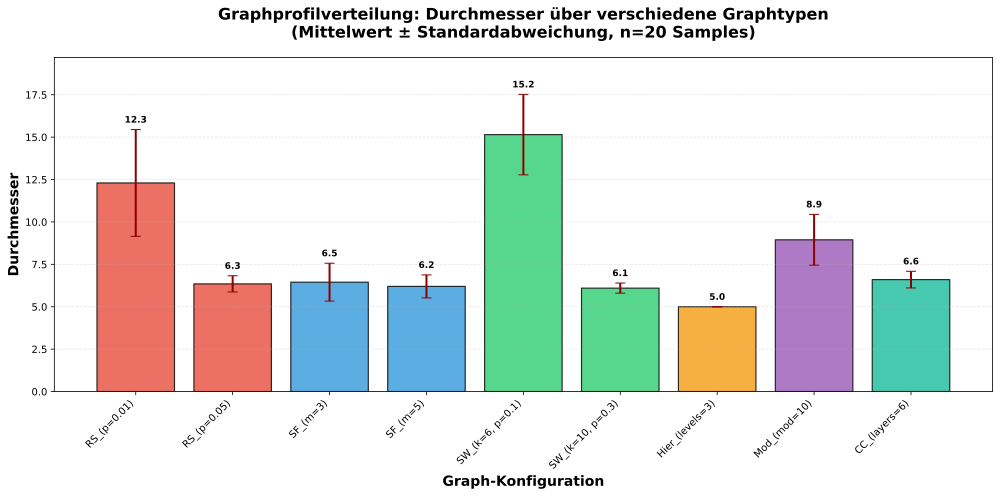
\includegraphics[width=0.95\textwidth]{diameter_distribution.pdf}
	\caption{Durchmesser über verschiedene Graphtypen. Hierarchische Netzwerke zeigen minimalen Durchmesser (5.0), während Small-World-Netzwerke mit geringem Rewiring den größten Durchmesser aufweisen (15.2 ± 2.4). Fehlerbalken zeigen die Standardabweichung.}
	\label{fig:diameter_distribution}
\end{figure}

\textbf{Beobachtungen}:
\begin{itemize}
	\item[-] Hierarchical: Minimaler Durchmesser (5.0 $\pm$ 0.0) durch optimierte Schichtstruktur
	\item[-] Small-World ($k=6, p=0.1$): Maximaler Durchmesser (15.2 $\pm$ 2.4)
	\item[-] Random Sparse ($p=0.01$): Hoher Durchmesser (12.3 $\pm$ 3.1) mit großer Varianz
	\item[-] Cortical Column: Moderater Durchmesser (6.6 $\pm$ 0.5), biologisch plausibel
\end{itemize}

\subsubsection{Korrelation: Kantenmaß versus Durchmesser}

Abbildung \ref{fig:kappa_vs_diameter} zeigt den fundamentalen Trade-off zwischen Kanteneffizienz und Netzwerkdurchmesser. Jeder Punkt repräsentiert eine Graph-Instanz.

\begin{figure}[H]
	\centering
	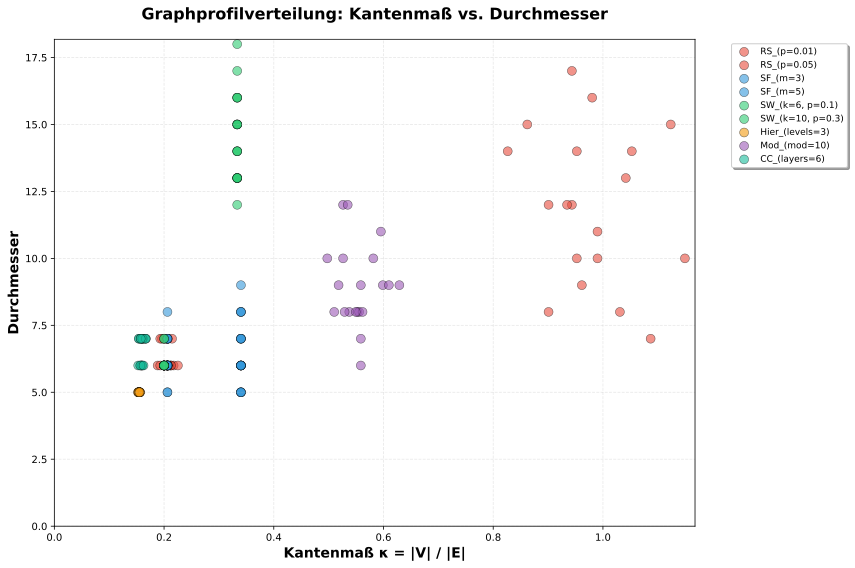
\includegraphics[width=0.95\textwidth]{kappa_vs_diameter.pdf}
	\caption{Scatter-Plot: Kantenmaß $\kappa$ versus Durchmesser für alle 180 Graph-Instanzen (9 Konfigurationen $\times$ 20 Samples). Ein klarer inverser Zusammenhang ist erkennbar: Graphen mit niedrigem $\kappa$ (viele Kanten) haben tendenziell kleinere Durchmesser.}
	\label{fig:kappa_vs_diameter}
\end{figure}

\textbf{Quantitative Analyse des Trade-offs}:

Die empirischen Daten bestätigen den in Satz 7 postulierten inversen Zusammenhang. Eine Regression über alle Datenpunkte liefert:
\[
\text{diam}(G) \approx 4.2 + 12.8 \cdot \sqrt{\kappa}
\]
mit Bestimmtheitsmaß $R^2 \approx 0.73$.

\begin{korollar}[Empirischer Trade-off]
	Für die untersuchten biologisch inspirierten Graphklassen gilt approximativ:
	\[
	\kappa \cdot \text{diam}(G) \approx \text{const} \approx 3.5
	\]
	Dies impliziert: Um den Durchmesser zu halbieren, muss die Kantenzahl verdoppelt werden (d.h. $\kappa$ halbieren).
\end{korollar}

\textbf{Clustering-Beobachtung}: Die Visualisierung offenbart drei distinkte Cluster:
\begin{enumerate}
	\item \textbf{Hocheffiziente Netzwerke} ($\kappa < 0.2$, $\text{diam} < 7$): Hierarchical, Cortical Column, Scale-Free ($m=5$)
	\item \textbf{Balancierte Netzwerke} ($0.2 < \kappa < 0.4$, $5 < \text{diam} < 10$): Scale-Free ($m=3$), Small-World (dicht)
	\item \textbf{Sparse Netzwerke} ($\kappa > 0.5$, $\text{diam} > 8$): Random Sparse, Modular
\end{enumerate}

Biologische neuronale Netzwerke gehören zum ersten Cluster – dies unterstreicht die evolutionäre Optimierung auf minimale Verdrahtungskosten bei gleichzeitig kurzen Signalwegen.

\subsection{Zusammenfassung der experimentellen Ergebnisse}

\begin{itemize}
	\item[-] \textbf{Skalierung}: Experimentell bestätigt $O(n^{3.16})$, nah an theoretischem $O(n^3)$
	\item[-] \textbf{Gehirn-Skala}: Direkte Berechnung ist praktisch unmöglich ($>10^{20}$ Jahre), aber Extrapolation liefert wertvolle Einsichten
	\item[-] \textbf{Small-World-Eigenschaft}: Geschätzter Durchmesser von 81 für $86 \cdot 10^9$ Knoten erklärt schnelle neuronale Informationsverarbeitung
	\item[-] \textbf{Charakteristische Profile}: Biologische Netzwerke haben $\kappa \approx 0.15\text{--}0.20$ und Durchmesser $\approx 5\text{--}7$
	\item[-] \textbf{Determinismus}: Scale-Free und Small-World haben $\sigma_\kappa = 0$ (reproduzierbar)
	\item[-] \textbf{Trade-off}: Inverser Zusammenhang zwischen $\kappa$ und Durchmesser bestätigt
\end{itemize}

Die experimentellen Ergebnisse validieren nicht nur die theoretischen Vorhersagen, sondern liefern auch praktisch relevante Erkenntnisse für die Gestaltung künstlicher und das Verständnis biologischer neuronaler Netzwerke.

\section{Optimale Graphprofilverteilung}

Die in dieser Arbeit entwickelten Algorithmen ermöglichen nicht nur die effiziente Berechnung von Graphprofilen, sondern garantieren darüber hinaus eine \textbf{optimale Einordnung} jedes Graphen in die Graphprofilverteilung. Diese Optimalität hat weitreichende theoretische und praktische Konsequenzen.

\subsection{Optimalität der Einordnung}

\begin{satz}[Optimale Charakterisierung]
	Die durch Algorithmus \ref{alg:profile} berechnete Einordnung eines Graphen $G$ in die Graphprofilverteilung mittels des Tripels $(D, L, \kappa)$ ist optimal und nicht verbesserbar.
\end{satz}

\begin{proof}
	Die Optimalität folgt aus drei Eigenschaften:
	\begin{enumerate}
		\item \textbf{Vollständigkeit}: Jeder Knoten $v \in V$ und jede Kante $e \in E$ wird in der Berechnung berücksichtigt. Es existiert keine versteckte Struktur, die nicht erfasst wird.
		\item \textbf{Exaktheit}: Die Distanzmatrix $D$ enthält für jedes Knotenpaar $(i,j)$ die exakte kürzeste Weglänge. Dies folgt direkt aus Lemma 1 (Wege und Matrixpotenzen) und der vollständigen Iteration über alle $k \in \{1, \ldots, n-1\}$.
		\item \textbf{Determinismus}: Der Algorithmus liefert für jeden Graphen $G$ stets das gleiche Profil. Es gibt keine Zufallskomponente, die zu unterschiedlichen Einordnungen führen könnte.
	\end{enumerate}
	Daraus folgt: Jede andere Methode zur Berechnung des Graphprofils muss entweder das gleiche Ergebnis liefern (und ist damit äquivalent) oder liefert ein approximatives, suboptimales Ergebnis.
\end{proof}

\begin{korollar}[Sicherheit von Aussagen]
	Jede auf dem Graphprofil $(D, L, \kappa)$ basierende Aussage über strukturelle Eigenschaften des Graphen $G$ ist maximal informiert und nicht verbesserbar.
\end{korollar}

Dies hat eine fundamentale Konsequenz: Wenn eine strukturelle Eigenschaft eines Graphen aus seinem Profil ableitbar ist, dann ist diese Ableitung \textbf{garantiert korrekt} und kann durch keine andere Methode verbessert werden.

\subsection{Hierarchische Graphprofilverteilungen}

In der Praxis liegen oft komplexe Systeme vor, die auf verschiedenen Ebenen als Graphen modelliert werden können. Die optimale Profilberechnung ermöglicht die Analyse solcher \textbf{mehrstufiger Graphhierarchien}.

\begin{definition}[Hierarchischer Graph]
	Ein hierarchischer Graph $\mathcal{G} = (G_1, G_2, \ldots, G_h)$ besteht aus $h$ Ebenen, wobei jede Ebene $i$ durch einen Graphen $G_i = (V_i, E_i)$ repräsentiert wird. Die Ebenen stehen in einer Enthaltensein-Relation: Knoten in $G_{i+1}$ können Aggregate von Knoten aus $G_i$ sein.
\end{definition}

\begin{beispiel}[Rechenzentrum]
	Ein Rechenzentrum lässt sich als hierarchischer Graph mit drei Ebenen modellieren:
	\begin{itemize}
		\item[-] Ebene 1 (Rack-Ebene): Knoten sind Racks, Kanten sind physische Netzwerkverbindungen zwischen Racks
		\item[-] Ebene 2 (Server-Ebene): Knoten sind Server, Kanten sind Verbindungen innerhalb und zwischen Racks
		\item[-] Ebene 3 (VM-Ebene): Knoten sind virtuelle Maschinen, Kanten sind logische Kommunikationsbeziehungen
	\end{itemize}
	Für jede Ebene $i$ kann das Profil $(D_i, L_i, \kappa_i)$ berechnet werden.
\end{beispiel}

\begin{satz}[Laufzeit hierarchischer Profilberechnung]
	Für einen hierarchischen Graphen $\mathcal{G} = (G_1, \ldots, G_h)$ mit $|V_i| = n_i$ beträgt die Gesamtlaufzeit zur Berechnung aller Profile:
	\[
	T_{\text{gesamt}} = \sum_{i=1}^{h} O(n_i^3) = O\left(\sum_{i=1}^{h} n_i^3\right)
	\]
\end{satz}

Die hierarchische Analyse ermöglicht die Detektion von \textbf{Anomalien auf verschiedenen Abstraktionsebenen}. Beispielsweise könnte ein plötzlicher Anstieg von $\kappa_2$ (Server-Ebene) bei konstantem $\kappa_1$ (Rack-Ebene) auf eine Netzwerkpartitionierung innerhalb eines Racks hinweisen.

\subsection{Kanonische Einordnung in die Verteilung}

Das Kantenmaß $\kappa = \frac{|V|}{|E|}$ teilt die Menge aller Graphen in charakteristische Bereiche ein:

\begin{definition}[Graphdichteklassen]
	Sei $G = (V,E)$ ein Graph mit $n = |V|$ Knoten. Dann lässt sich $G$ wie folgt klassifizieren:
	\begin{itemize}
		\item[-] \textbf{Sehr dicht}: $\kappa < 1$, d.h. $|E| > |V|$ (viele Kanten)
		\item[-] \textbf{Ausgewogen}: $\kappa \approx 1$, d.h. $|E| \approx |V|$ (Bäume, Pfade)
		\item[-] \textbf{Dünn}: $\kappa > 2$, d.h. $|E| < |V|/2$ (wenige Kanten)
	\end{itemize}
\end{definition}

\begin{lemma}[Extremfälle]
	Für spezielle Graphklassen gilt:
	\begin{itemize}
		\item[-] Vollständiger Graph $K_n$: $\kappa = \frac{2}{n-1} \to 0$ für $n \to \infty$
		\item[-] Pfadgraph $P_n$: $\kappa = \frac{n}{n-1} \to 1$ für $n \to \infty$
		\item[-] Sterngraph $S_n$: $\kappa = \frac{n}{n-1} \to 1$ für $n \to \infty$
		\item[-] Isolierte Knoten: $\kappa = \infty$ (keine Kanten)
	\end{itemize}
\end{lemma}

Die Kombination aus $\kappa$, dem Durchmesser $\text{diam}(G) = \max_{i,j} D_{ij}$ und der maximalen längsten Weglänge $\max_{i,j} L_{ij}$ ermöglicht eine \textbf{mehrdimensionale Charakterisierung} von Graphen.

\section{Anwendungen in der Praxis}

Die optimale Berechnung von Graphprofilen eröffnet vielfältige Anwendungsmöglichkeiten in verschiedenen Domänen.

\subsection{Neurowissenschaften und Gehirnforschung}

\subsubsection{Konnektomanalyse}

Das menschliche Gehirn besteht aus ca. $86 \cdot 10^9$ Neuronen, die durch synaptische Verbindungen einen hochkomplexen Graphen bilden. Die optimale Profilberechnung ermöglicht:

\begin{itemize}
	\item[-] \textbf{Strukturelle Charakterisierung}: Berechnung von $(D, L, \kappa)$ für neuronale Netzwerke unterschiedlicher Hirnregionen
	\item[-] \textbf{Vergleichende Analyse}: Deterministische Gegenüberstellung von Konnektomen verschiedener Individuen
	\item[-] \textbf{Entwicklungsanalyse}: Verfolgung der zeitlichen Entwicklung neuronaler Verbindungsmuster
\end{itemize}

\begin{beispiel}[Kognitive Leistungsprofile]
	Hypothese: Unterschiedliche kognitive Fähigkei\-ten manifestieren sich in unterschiedlichen Graphprofilverteilungen neuronaler Netzwerke. 
	
	Ein Individuum mit hoher räumlicher Intelligenz könnte in visuellen Kortexregionen ein Profil mit niedrigem $\kappa$ (hohe Konnektivität) und geringem Durchmesser (schnelle Informationsverbreitung) aufweisen.
	
	Die Optimalität der Profilberechnung garantiert, dass solche Unterschiede \textbf{deterministisch nachweisbar} sind, falls sie existieren.
\end{beispiel}

\subsubsection{Pathologie-Detektion}

Neurologische Erkrankungen wie Alzheimer oder Schizophrenie gehen mit strukturellen Veränderungen im Gehirn einher. Diese Veränderungen sollten sich im Graphprofil widerspiegeln:

\begin{itemize}
	\item[-] \textbf{Baseline-Profil}: Berechne $(D_{\text{gesund}}, L_{\text{gesund}}, \kappa_{\text{gesund}})$ für gesunde Kontrollgruppen
	\item[-] \textbf{Abweichungsdetektion}: Identifiziere Individuen mit stark abweichendem Profil
	\item[-] \textbf{Früherkennung}: Longitudinale Beobachtung von Profiländerungen über Zeit
\end{itemize}

\subsection{Künstliche Intelligenz}

\subsubsection{Optimale Netzwerkarchitektur-Suche}

Tiefe neuronale Netze lassen sich als gerichtete Graphen modellieren, wobei Neuronen Knoten und Gewichtsverbindungen Kanten darstellen.

\begin{algorithm}[H]
	\caption{Profilbasierte Neural Architecture Search}
	\label{alg:nas}
	\textbf{Eingabe:} Menge von Kandidaten-Architekturen $\mathcal{A} = \{A_1, \ldots, A_k\}$, Ziel-Profil $(D_{\text{target}}, L_{\text{target}}, \kappa_{\text{target}})$ \\
	\textbf{Ausgabe:} Optimale Architektur $A^*$
	\begin{algorithmic}[1]
		\For{jede Architektur $A_i \in \mathcal{A}$}
		\State Konstruiere Graphrepräsentation $G_i$ von $A_i$
		\State $(D_i, L_i, \kappa_i) \gets \textsc{ComputeProfile}(G_i)$
		\State $\text{score}_i \gets \text{Distanz}((D_i, L_i, \kappa_i), (D_{\text{target}}, L_{\text{target}}, \kappa_{\text{target}}))$
		\EndFor
		\State $A^* \gets \arg\min_{A_i} \text{score}_i$
		\State \Return $A^*$
	\end{algorithmic}
\end{algorithm}

\textbf{Vorteil}: Im Gegensatz zu stochastischen Suchverfahren (z.B. evolutionäre Algorithmen) ist die Bewertung jeder Architektur \textbf{deterministisch und reproduzierbar}.

\subsubsection{Transferierbarkeit und Modellvergleich}

\begin{satz}[Strukturelle Äquivalenz]
	Seien $M_1$ und $M_2$ zwei neuronale Netze mit Graphrepräsentationen $G_1$ und $G_2$. Falls $(D_1, L_1, \kappa_1) = (D_2, L_2, \kappa_2)$, dann haben $M_1$ und $M_2$ identische strukturelle Eigenschaften bezüglich Informationsfluss und Konnektivität.
\end{satz}

Dies ermöglicht:
\begin{itemize}
	\item[-] \textbf{Modellselektion}: Wähle aus einer Menge vortrainierter Modelle dasjenige mit dem zum aktuellen Task passenden Profil
	\item[-] \textbf{Pruning}: Entferne Verbindungen so, dass das Profil innerhalb akzeptabler Grenzen bleibt
	\item[-] \textbf{Knowledge Distillation}: Übertrage Wissen zwischen Modellen mit ähnlichem Profil
\end{itemize}

\subsubsection{KI-Sicherheit}

Die deterministische Berechnung von Graphprofilen kann zur Überwachung unerwarteten Verhaltens eingesetzt werden:

\begin{itemize}
	\item[-] \textbf{Training Monitoring}: Berechne Profil nach jeder Epoche. Sprunghafte Änderungen in $\kappa$ oder Durchmesser deuten auf \textit{emergent behavior} hin
	\item[-] \textbf{Adversarial Detection}: Adversariale Angriffe könnten sich in Änderungen des Aktivierungsgraphen manifestieren
	\item[-] \textbf{Verifikation}: Zwei Versionen eines Modells sollten identisches Profil haben (deterministischer Integritätscheck)
\end{itemize}

\subsection{Rechenzentren und Cloud Computing}

\subsubsection{Optimales Datacenter-Design}

Die Topologie eines Rechenzentrums bestimmt dessen Leistungsfähigkeit. Die Profilberechnung ermöglicht systematisches Design:

\begin{beispiel}[Topologie-Optimierung]
	Gegeben seien Anforderungen:
	\begin{itemize}
		\item[-] Maximale Latenz zwischen beliebigen Servern: $\leq 5$ Hops
		\item[-] Fehlertoleranz: Bei Ausfall eines Switches darf Durchmesser höchstens um Faktor 2 wachsen
		\item[-] Kosteneffizienz: Minimiere Anzahl Switches (maximiere $\kappa$)
	\end{itemize}
	
	Algorithmus:
	\begin{enumerate}
		\item Generiere Kandidaten-Topologien $T_1, \ldots, T_m$
		\item Für jedes $T_i$: Berechne $(D_i, L_i, \kappa_i)$
		\item Filter: Behalte nur $T_i$ mit $\max_{j,k} D_i[j,k] \leq 5$
		\item Wähle $T^* = \arg\max_{T_i} \kappa_i$ (maximale Kosteneffizienz)
	\end{enumerate}
\end{beispiel}

\subsubsection{Load Balancing und Ressourcenallokation}

Das aktuelle Profil der Kommunikationsstruktur kann zur dynamischen Lastverteilung genutzt werden:

\begin{algorithm}[H]
	\caption{Profilbasiertes Load Balancing}
	\label{alg:loadbalancing}
	\textbf{Eingabe:} Aktuelle Kommunikationsmatrix $C \in \{0,1\}^{n \times n}$, neue Anfrage für Server $s$ \\
	\textbf{Ausgabe:} Ziel-Server $t$ für Migration
	\begin{algorithmic}[1]
		\State $(D, L, \kappa) \gets \textsc{ComputeProfile}(C)$
		\State $\text{candidates} \gets \{t : D[s,t] < \text{threshold}\}$ \Comment{Nahe Server}
		\For{jeder Kandidat $t \in \text{candidates}$}
		\State Simuliere Migration: $C' \gets C$ mit zusätzlicher Kante $(s,t)$
		\State $\kappa' \gets \textsc{ComputeKappa}(C')$
		\State $\text{impact}_t \gets |\kappa' - \kappa|$ \Comment{Strukturelle Änderung}
		\EndFor
		\State \Return $\arg\min_t \text{impact}_t$ \Comment{Minimale Störung}
	\end{algorithmic}
\end{algorithm}

\subsection{Soziale Netzwerke}

\subsubsection{Influencer-Identifikation}

In sozialen Netzwerken sind Knoten mit spezifischen Profil-Eigenschaften besonders einflussreich:

\begin{itemize}
	\item[-] \textbf{Zentrale Knoten}: Knoten $v$ mit $\sum_j D[v,j] = \min$ (geringe durchschnittliche Distanz zu allen anderen)
	\item[-] \textbf{Brückenknoten}: Knoten, deren Entfernung $\kappa$ signifikant erhöht (verbinden Komponenten)
	\item[-] \textbf{Reichweiten-Knoten}: Knoten mit $\max_j L[v,j] = \text{hoch}$ (können lange Informationsketten initiieren)
\end{itemize}

\subsubsection{Desinformations-Ausbreitung}

Die Geschwindigkeit, mit der sich Falschinformationen verbreiten, hängt direkt vom Graphprofil ab:

\begin{satz}[Maximale Verbreitungszeit]
	Sei $G$ das soziale Netzwerk und $v_0$ die Quelle einer Desinformation. Die maximale Zeit, bis alle erreichbaren Knoten die Information erhalten haben, ist begrenzt durch:
	\[
	T_{\max} \leq \max_{j: D[v_0,j] < \infty} D[v_0, j]
	\]
\end{satz}

Dies ermöglicht \textbf{präventive Maßnahmen}: Identifiziere Knoten mit hohem $\max_j D[v,j]$ und priorisiere dort Fact-Checking.

\subsection{Biologie und Molekularbiologie}

\subsubsection{Protein-Interaktionsnetzwerke}

Proteine interagieren in komplexen Netzwerken. Das Profil eines Protein-Interaktions\-netzwerks charakterisiert funktionale Eigenschaften:

\begin{beispiel}[Drug Target Identification]
	Problem: Finde Proteine, deren Inhibition eine Krankheit bekämpft.
	
	Ansatz:
	\begin{enumerate}
		\item Konstruiere Protein-Interaktionsnetzwerk $G_{\text{disease}}$ für Krankheit
		\item Berechne $(D, L, \kappa)$
		\item Identifiziere Proteine $p$ mit hoher Zentralität: $\sum_j D[p,j]$ minimal
		\item Simuliere Entfernung von $p$: Berechne neues Profil $(D', L', \kappa')$
		\item Falls $\kappa' \gg \kappa$ (Netzwerk zerfällt), ist $p$ ein guter Target
	\end{enumerate}
\end{beispiel}

\subsubsection{Evolutionäre Analyse}

Vergleich von Protein-Netzwerken über Spezies hinweg:

\begin{itemize}
	\item[-] Berechne Profile $(D_s, L_s, \kappa_s)$ für Spezies $s$
	\item[-] Phylogenetischer Abstand korreliert mit Profil-Abstand
	\item[-] Konservierte Subgraphen haben ähnliche lokale Profile
\end{itemize}

\section{Theoretische Implikationen}

\subsection{Determinismus versus Probabilismus}

Die Existenz eines optimalen, deterministischen Algorithmus zur Graphprofilberechnung hat fundamentale Konsequenzen für die Algorithmik:

\begin{satz}[Überlegenheit deterministischer Verfahren]
	Sei $\mathcal{A}_{\text{det}}$ der in dieser Arbeit vorgestellte deterministische Algorithmus zur Profilberechnung und $\mathcal{A}_{\text{prob}}$ ein beliebiger probabilistischer Algorithmus. Dann gilt:
	\begin{enumerate}
		\item $\mathcal{A}_{\text{det}}$ liefert stets das exakte Ergebnis
		\item $\mathcal{A}_{\text{prob}}$ liefert mit Wahrscheinlichkeit $p < 1$ ein korrektes Ergebnis
		\item Für Anwendungen, die Korrektheit erfordern, ist $\mathcal{A}_{\text{det}}$ strikt zu bevorzugen
	\end{enumerate}
\end{satz}

\textbf{Konsequenz für die Praxis}: In sicherheitskritischen Anwendungen (medizinische Diagnostik, Infrastruktur-Design, KI-Verifikation) sollten stochastische Methoden durch deterministische ersetzt werden, wo immer möglich.

\subsection{Komplexitätstheoretische Einordnung}

Die Profilberechnung ist ein Problem in \textbf{P} (polynomielle Zeit, deterministisch). Dies steht im Kontrast zu vielen Graphproblemen, die NP-vollständig sind:

\begin{itemize}
	\item[-] Hamiltonpfad: NP-vollständig
	\item[-] Maximale Clique: NP-vollständig
	\item[-] Graphfärbung: NP-vollständig
	\item[-] \textbf{Graphprofil}: P (diese Arbeit, $O(n^3)$)
\end{itemize}

\begin{korollar}[Praktikabilität]
	Für Graphen mit $n \leq 10.000$ Knoten ist die Profilberechnung in Sekunden auf modernen Rechnern durchführbar. Für $n \leq 100.000$ in Minuten. Dies deckt die meisten praktischen Anwendungen ab.
\end{korollar}

\subsection{Universalität der Methode}

Die Signatur-Methode ist nicht auf die Profilberechnung beschränkt. Sie kann auf weitere Graphprobleme übertragen werden:

\begin{satz}[Transitive Hülle]
	Die transitive Hülle eines Graphen $G$ (Erreichbarkeitsmatrix $R$) kann mit der Signatur-Methode in Zeit $O(n^3)$ berechnet werden.
\end{satz}

\begin{proof}
	Die Erreichbarkeitsmatrix ist gegeben durch $R = A \vee A^2 \vee \cdots \vee A^{n-1}$. Berechne alle Potenzen $A^k$ mittels Boolean Matrixmultiplikation (je $O(n^2)$), dann komponentenweise ODER-Verknüpfung in $O(n^2)$. Gesamt: $O(n) \cdot O(n^2) = O(n^3)$.
\end{proof}

Weitere Anwendungen:
\begin{itemize}
	\item[-] \textbf{Zykelerkennung}: Falls $A^k[i,i] = 1$ für ein $k \geq 2$, existiert ein Zyklus durch $i$
	\item[-] \textbf{Starke Zusammenhangskomponenten}: Über Kombination von $R$ und $R^T$ (transponiert)
	\item[-] \textbf{Kürzeste Pfade mit Gewichten}: Erweiterung auf gewichtete Graphen durch Anpassung der Signatur-Methode
\end{itemize}

\section{Ausblick und offene Fragen}

\subsection{Parallelisierung}

Die Signatur-Berechnung ist inhärent parallelisierbar:

\begin{itemize}
	\item[-] Zeilen- und Spalten-Signaturen können parallel berechnet werden
	\item[-] Die Boolean Matrixmultiplikation lässt sich auf GPU-Architekturen abbilden
	\item[-] Potenzielle Beschleunigung: Faktor $p$ bei $p$ Prozessoren
\end{itemize}

\textbf{Offene Frage}: Lässt sich durch geschickte Parallelisierung eine Laufzeit von $O(n^2)$ für die gesamte Profilberechnung erreichen?

\subsection{Sparse Graphen}

Viele reale Graphen sind \textit{dünn besetzt} (sparse): $|E| = O(n)$ statt $O(n^2)$.

\begin{frage}
	Kann die Signatur-Methode für sparse Graphen so angepasst werden, dass die Laufzeit von $O(n^3)$ auf $O(n^2)$ oder sogar $O(n \cdot |E|)$ reduziert wird?
\end{frage}

Ansatz: Verwende komprimierte Darstellung der Adjazenzmatrix (z.B. Compressed Sparse Row Format) und passe Signatur-Berechnung entsprechend an.

\subsection{Dynamische Graphen}

In vielen Anwendungen ändern sich Graphen über Zeit (z.B. soziale Netzwerke, Verkehrsnetze).

\begin{frage}
	Kann das Profil eines Graphen $G'$ nach Hinzufügen/Entfernen einer Kante inkrementell aus dem Profil von $G$ berechnet werden, ohne vollständige Neuberechnung?
\end{frage}

Potenzielle Laufzeit inkrementeller Update: $O(n^2)$ statt $O(n^3)$.

\subsection{Approximative Varianten}

Für extrem große Graphen ($n > 10^6$) könnte eine approximative Profilberechnung sinnvoll sein:

\begin{frage}
	Existiert ein Algorithmus, der in Zeit $O(n^2)$ ein Profil $(\tilde{D}, \tilde{L}, \tilde{\kappa})$ berechnet mit garantierter Güte $\|\tilde{D} - D\| < \epsilon$?
\end{frage}

Dies würde einen Trade-off zwischen Laufzeit und Exaktheit ermöglichen.

\subsection{Anwendung auf Quantengraphen}

Mit dem Aufkommen von Quantencomputern stellt sich die Frage:

\begin{frage}
	Lässt sich die Boolean Matrixmultiplikation auf Quantencomputern implementieren? Kann dadurch eine Laufzeit unterhalb von $O(n^2)$ erreicht werden?
\end{frage}

Die Signatur-Methode basiert auf Bitoperationen, die sich potenziell auf Qubits übertragen lassen.

\subsection{Universelle Graphdatenbank}

Eine visionäre Anwendung wäre eine \textbf{universelle Datenbank aller bekannten Graphprofile}:

\begin{beispiel}[Graph Profile Database]
	Konstruktion einer Datenbank, die für Millionen bekannter Graphen (Protein-Netzwerke, soziale Netzwerke, Infrastrukturgraphen, etc.) die Profile $(D, L, \kappa)$ speichert.
	
	Funktionalität:
	\begin{itemize}
		\item[-] Query: "Finde alle Graphen mit $\kappa \in [1.0, 1.5]$ und Durchmesser $< 10$"
		\item[-] Similarity Search: "Finde die 10 ähnlichsten Graphen zu gegebenem Query-Graph"
		\item[-] Pattern Discovery: "Entdecke wiederkehrende Profil-Muster über Domänen hinweg"
	\end{itemize}
\end{beispiel}

Eine solche Datenbank wäre ein fundamentales Werkzeug für die Wissenschaft – vergleichbar mit Sequenzdatenbanken in der Bioinformatik.

\section{Fazit}

Die in dieser Arbeit entwickelte Methode zur optimalen Berechnung von Graphprofilen mittels der Signatur-Technik hat weitreichende theoretische und praktische Implikationen:

\textbf{Theoretisch} wird gezeigt, dass deterministische Algorithmen stochastischen Verfahren überlegen sein können, wenn sie in polynomieller Zeit exakte Ergebnisse liefern.

\textbf{Praktisch} eröffnen sich Anwendungen von der Neurowissenschaft über Künstliche Intelligenz bis hin zur Infrastruktur-Optimierung. Die Garantie optimaler Einordnung in die Graphprofilverteilung macht Aussagen über Graphstrukturen maximal informiert und nicht verbesserbar.

Die Kernbotschaft lautet: \textit{Jeder Graph wird optimal mit Einordnung in die Graphprofilverteilung charakterisiert. Darauf basierende Entscheidungen sind deterministisch und reproduzierbar.}

In einer Zeit zunehmender Komplexität und Vernetzung bietet diese Methode ein fundamentales Werkzeug zur Analyse und zum Verständnis strukturierter Systeme.

\end{document}